% Options for packages loaded elsewhere
\PassOptionsToPackage{unicode}{hyperref}
\PassOptionsToPackage{hyphens}{url}
\PassOptionsToPackage{dvipsnames,svgnames,x11names}{xcolor}
%
\documentclass[
  letterpaper,
  DIV=11,
  numbers=noendperiod]{scrartcl}

\usepackage{amsmath,amssymb}
\usepackage{iftex}
\ifPDFTeX
  \usepackage[T1]{fontenc}
  \usepackage[utf8]{inputenc}
  \usepackage{textcomp} % provide euro and other symbols
\else % if luatex or xetex
  \usepackage{unicode-math}
  \defaultfontfeatures{Scale=MatchLowercase}
  \defaultfontfeatures[\rmfamily]{Ligatures=TeX,Scale=1}
\fi
\usepackage{lmodern}
\ifPDFTeX\else  
    % xetex/luatex font selection
\fi
% Use upquote if available, for straight quotes in verbatim environments
\IfFileExists{upquote.sty}{\usepackage{upquote}}{}
\IfFileExists{microtype.sty}{% use microtype if available
  \usepackage[]{microtype}
  \UseMicrotypeSet[protrusion]{basicmath} % disable protrusion for tt fonts
}{}
\makeatletter
\@ifundefined{KOMAClassName}{% if non-KOMA class
  \IfFileExists{parskip.sty}{%
    \usepackage{parskip}
  }{% else
    \setlength{\parindent}{0pt}
    \setlength{\parskip}{6pt plus 2pt minus 1pt}}
}{% if KOMA class
  \KOMAoptions{parskip=half}}
\makeatother
\usepackage{xcolor}
\setlength{\emergencystretch}{3em} % prevent overfull lines
\setcounter{secnumdepth}{-\maxdimen} % remove section numbering
% Make \paragraph and \subparagraph free-standing
\ifx\paragraph\undefined\else
  \let\oldparagraph\paragraph
  \renewcommand{\paragraph}[1]{\oldparagraph{#1}\mbox{}}
\fi
\ifx\subparagraph\undefined\else
  \let\oldsubparagraph\subparagraph
  \renewcommand{\subparagraph}[1]{\oldsubparagraph{#1}\mbox{}}
\fi


\providecommand{\tightlist}{%
  \setlength{\itemsep}{0pt}\setlength{\parskip}{0pt}}\usepackage{longtable,booktabs,array}
\usepackage{calc} % for calculating minipage widths
% Correct order of tables after \paragraph or \subparagraph
\usepackage{etoolbox}
\makeatletter
\patchcmd\longtable{\par}{\if@noskipsec\mbox{}\fi\par}{}{}
\makeatother
% Allow footnotes in longtable head/foot
\IfFileExists{footnotehyper.sty}{\usepackage{footnotehyper}}{\usepackage{footnote}}
\makesavenoteenv{longtable}
\usepackage{graphicx}
\makeatletter
\def\maxwidth{\ifdim\Gin@nat@width>\linewidth\linewidth\else\Gin@nat@width\fi}
\def\maxheight{\ifdim\Gin@nat@height>\textheight\textheight\else\Gin@nat@height\fi}
\makeatother
% Scale images if necessary, so that they will not overflow the page
% margins by default, and it is still possible to overwrite the defaults
% using explicit options in \includegraphics[width, height, ...]{}
\setkeys{Gin}{width=\maxwidth,height=\maxheight,keepaspectratio}
% Set default figure placement to htbp
\makeatletter
\def\fps@figure{htbp}
\makeatother

\KOMAoption{captions}{tableheading}
\makeatletter
\@ifpackageloaded{caption}{}{\usepackage{caption}}
\AtBeginDocument{%
\ifdefined\contentsname
  \renewcommand*\contentsname{Table of contents}
\else
  \newcommand\contentsname{Table of contents}
\fi
\ifdefined\listfigurename
  \renewcommand*\listfigurename{List of Figures}
\else
  \newcommand\listfigurename{List of Figures}
\fi
\ifdefined\listtablename
  \renewcommand*\listtablename{List of Tables}
\else
  \newcommand\listtablename{List of Tables}
\fi
\ifdefined\figurename
  \renewcommand*\figurename{Figure}
\else
  \newcommand\figurename{Figure}
\fi
\ifdefined\tablename
  \renewcommand*\tablename{Table}
\else
  \newcommand\tablename{Table}
\fi
}
\@ifpackageloaded{float}{}{\usepackage{float}}
\floatstyle{ruled}
\@ifundefined{c@chapter}{\newfloat{codelisting}{h}{lop}}{\newfloat{codelisting}{h}{lop}[chapter]}
\floatname{codelisting}{Listing}
\newcommand*\listoflistings{\listof{codelisting}{List of Listings}}
\makeatother
\makeatletter
\makeatother
\makeatletter
\@ifpackageloaded{caption}{}{\usepackage{caption}}
\@ifpackageloaded{subcaption}{}{\usepackage{subcaption}}
\makeatother
\ifLuaTeX
  \usepackage{selnolig}  % disable illegal ligatures
\fi
\usepackage{bookmark}

\IfFileExists{xurl.sty}{\usepackage{xurl}}{} % add URL line breaks if available
\urlstyle{same} % disable monospaced font for URLs
\hypersetup{
  pdftitle={London SDE/AIC Programme: Introduction and Proposed Use-Cases},
  colorlinks=true,
  linkcolor={blue},
  filecolor={Maroon},
  citecolor={Blue},
  urlcolor={Blue},
  pdfcreator={LaTeX via pandoc}}

\title{London SDE/AIC Programme: Introduction and Proposed Use-Cases}
\author{Dr.~Joe Zhang \emph{(Head of Data Science)} \and Prof.~James Teo
\emph{(Clinical Director AI \& Data)} \and Dr.~Jorge Cardoso
\emph{(Chief Technology Officer)} \and Jawad Chaudhry \emph{(AI
Programme Lead)} \and Sigal Hachlili \emph{(Director of AI, Data \&
Digital)}}
\date{}

\begin{document}
\maketitle

\emph{Version 0.9 (last updated 2024 Apr 30)}

\subsection{Introduction}\label{introduction}

The \href{https://www.aicentre.co.uk/}{London AI Centre} (AIC) has been
commissioned as part of the London Secure Data Environment (SDE)
programme for its latest phase: to extend AI technologies and analytics
capabilities to stakeholders and data environments across London. This
document summarises the latest state of planning for the programme, as
an aid to internal and external stakeholders including Integrated Care
Boards (ICB) and the wider London NHS ecosystem.

\subsection{What is the London SDE?}\label{what-is-the-london-sde}

The London Secure Data Environment (SDE) is part of a national programme
to enable secure and more powerful analytics for NHS, academic, and
commercial users. Uniquely amongst regional peers, the London SDE does
not focus on a single research platform. Rather, it places a focus on
developing data infrastructure and capabilities across the region to
support population health, care providers, and commissioners. This is in
addition to building data environments that enable commercial research
and development partnerships.

The SDE is led by \textbf{OneLondon}, as part of an overarching London
Health Data Strategy, coalescing around three components
(Figure~\ref{fig-sde-summary}):

\begin{enumerate}
\def\labelenumi{(\arabic{enumi})}
\item
  \textbf{London Data Service (LDS)}: hosted in North-East London, the
  LDS serves as a data engineering and service layer for pan-London
  primary care and secondary care data. It handles data extraction and
  linkage, and provisions data within secure analytics environments for
  both research and NHS users.
\item
  \textbf{DiscoverNOW Research/Analytics Environment}: run by Imperial
  College Healthcare Partners in North-West London, DiscoverNOW supports
  governance and operation of secure research environments for academic,
  commercial, and NHS research and analytics.
\item
  \textbf{London AI Centre (AIC)}: a national centre of excellence for
  applied data science and AI, the AIC provides frontier technology for
  data enrichment (CogStack), federated analytics (FLIP), and deployment
  of machine learning tools, as well as expertise in health data and
  advanced analytics.
\end{enumerate}

\begin{figure}

\centering{

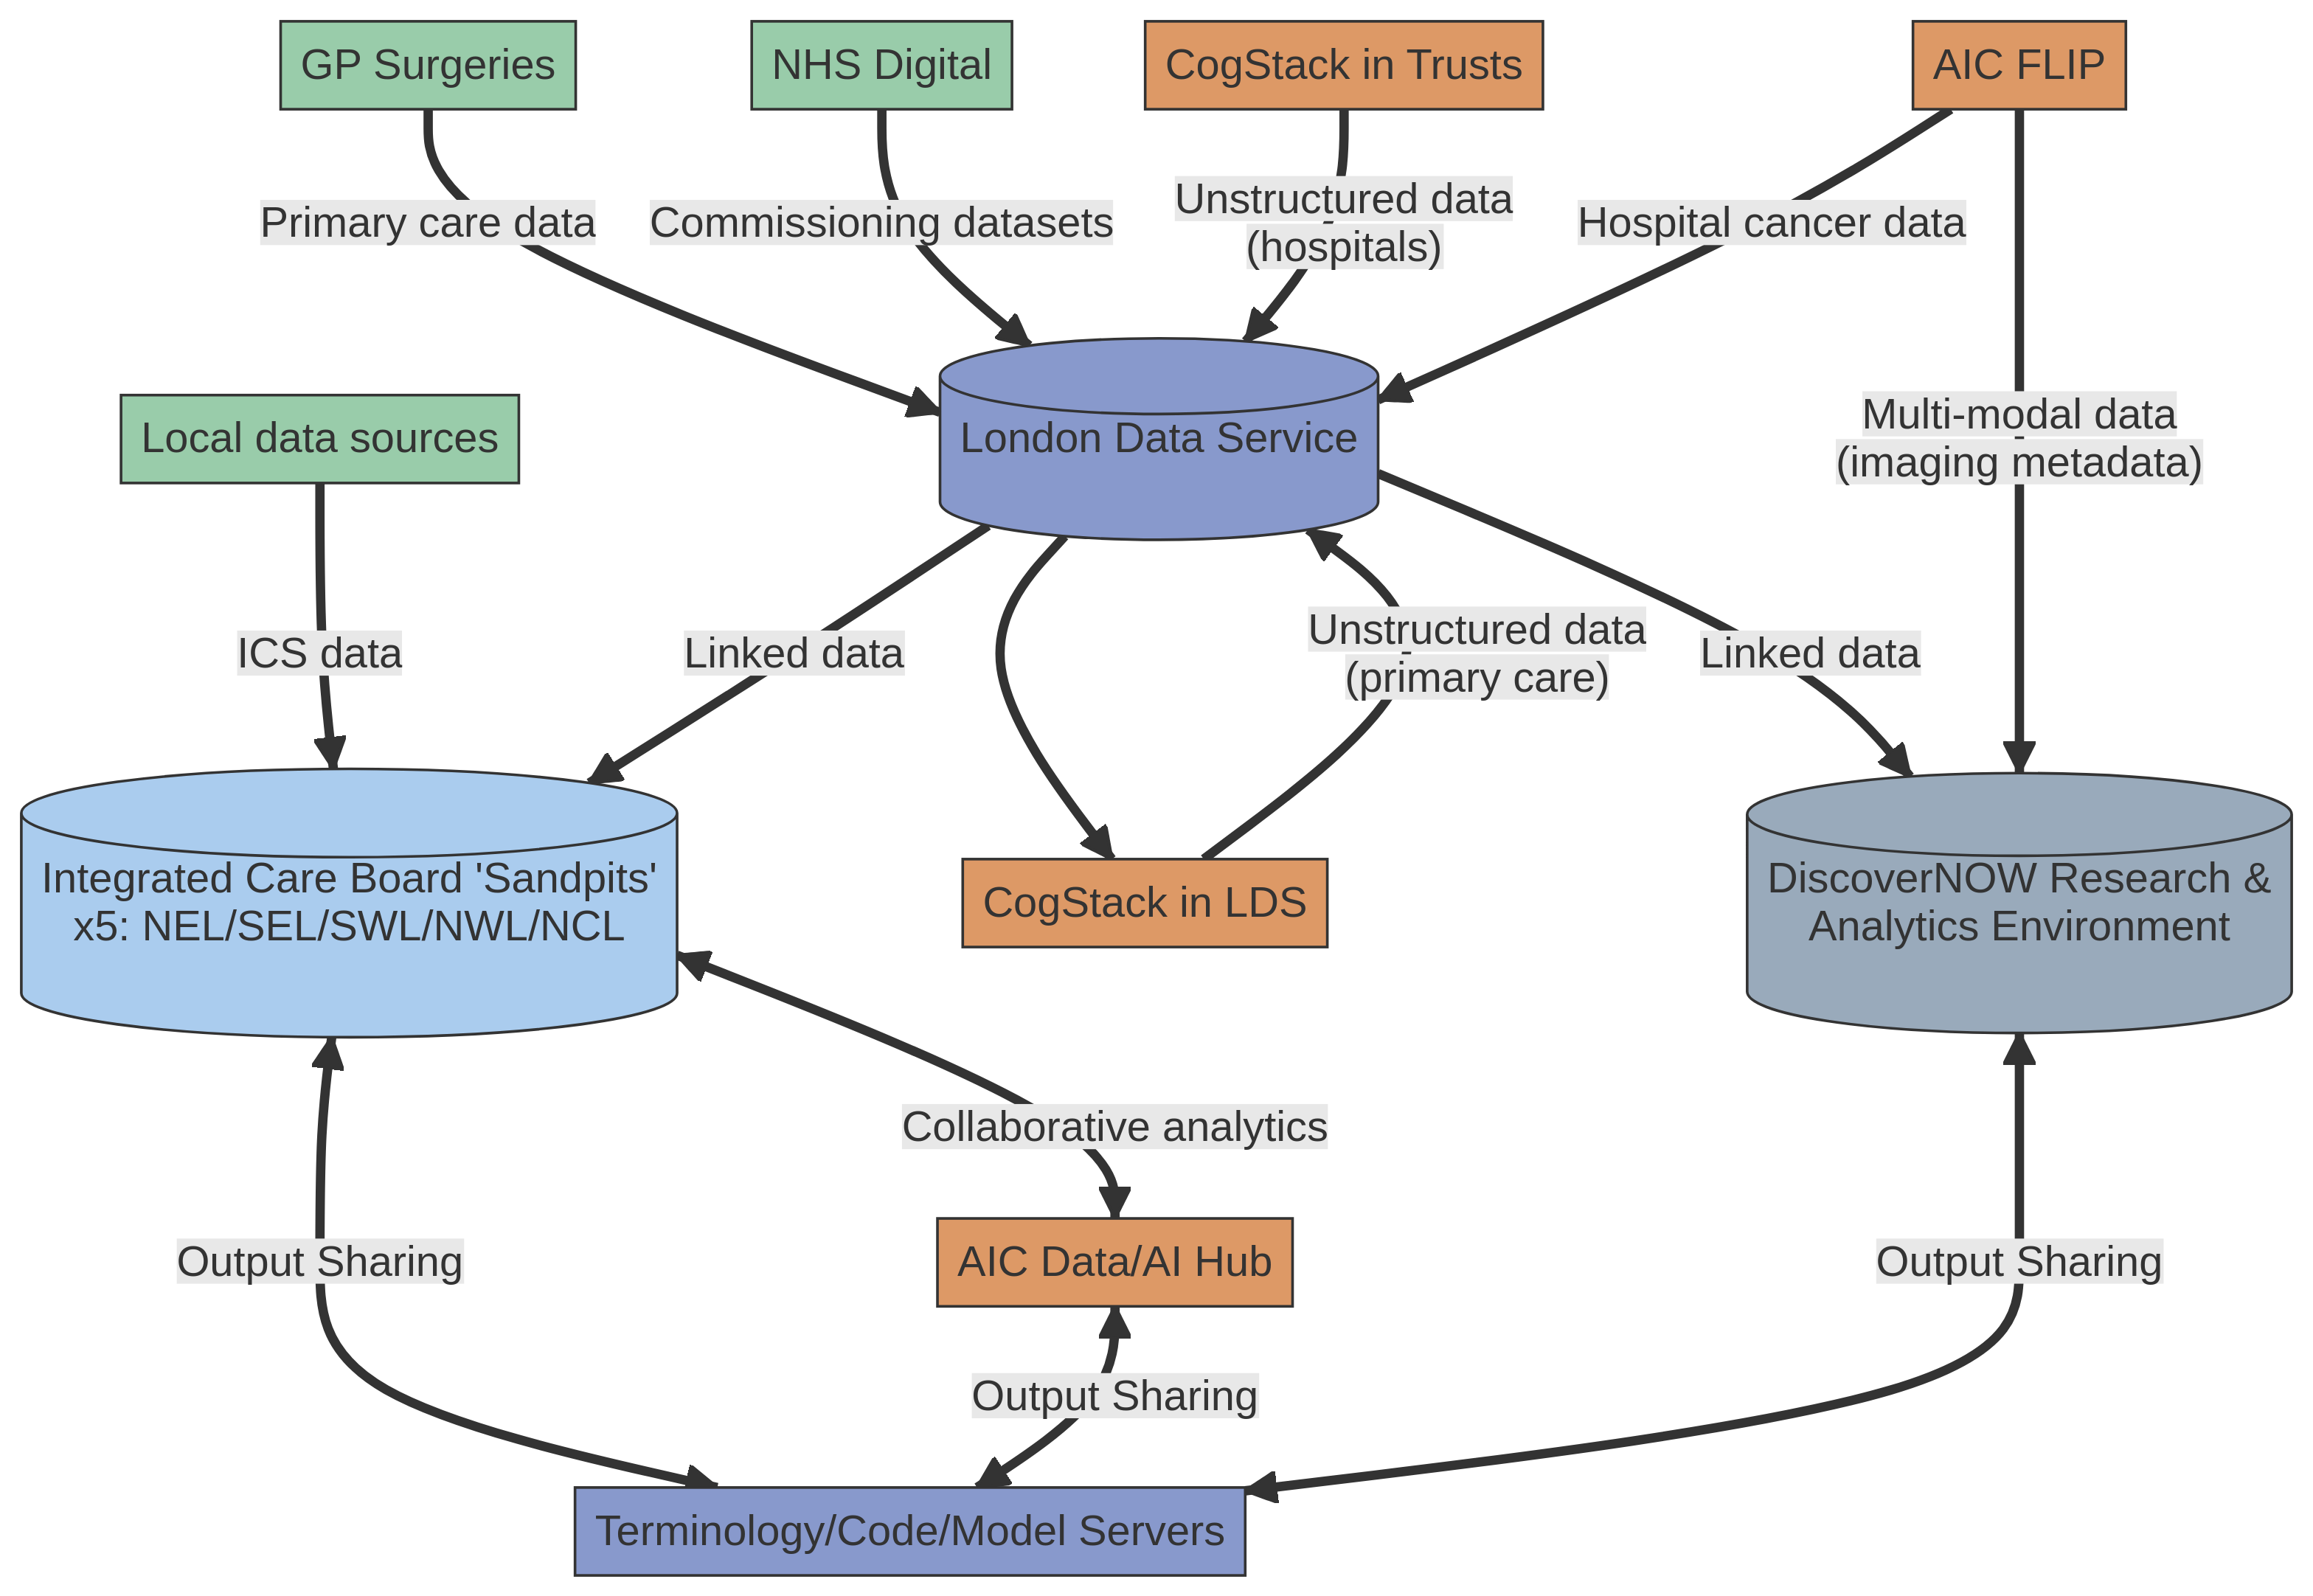
\includegraphics[width=6in,height=4.14in]{index_files/figure-latex/mermaid-figure-5.png}

}

\caption{\label{fig-sde-summary}Summary of SDE components and data
flows. Each London ICB is provisioned with its own data/analytics
environment through the LDS. FLIP = Federated Learning and
Interoperability Platform.}

\end{figure}%

\textsubscript{Source:
\href{https://d3london.github.io/sde_aic_docs/index.qmd.html}{Article
Notebook}}

\subsection{Technology and objectives}\label{technology-and-objectives}

The contribution from the London AIC consists of technology deployment
and supporting expertise, that enable a number of objectives
(Figure~\ref{fig-aic-objectives}) over the two year programme. This
contribution includes the following:

\begin{enumerate}
\def\labelenumi{(\arabic{enumi})}
\item
  \textbf{Federated Learning and Interoperability Platform (FLIP)}: FLIP
  consists of (a) secure data environments within NHS hospital Trusts
  for multi-modal imaging data, imaging metadata, and structured health
  record data in the OMOP common data model; and (b) a mechanism to
  query data and train AI models across these secure enclaves without
  the need to physically transfer data. FLIP is presently installed in
  four major London Trusts. Integrating FLIP into the SDE will enable
  hospital data (such as cancer data) to be surfaced into the LDS, and
  enable access to multi-modal data (such as DICOM imaging and digital
  pathology) for research in precision healthcare.
\item
  \textbf{CogStack}: As an advanced natural language processing
  platform, CogStack can turn the large quantities of health information
  that are found in narrative text, into structured and analysable data.
  Currently actively used in Trusts to assist with clinical coding from
  notes and clinic letters, CogStack can surface secondary care and
  cancer pathway data, and previously unseen primary care data, into the
  SDE ecosystem.
\item
  \textbf{AIC Data/AI Hub}: The AIC hosts substantial health data and AI
  implementation expertise, that will provide practical support in data
  engineering, clinical informatics, data science, and machine learning
  (ML) development and deployment. Primary aims are to (a) help
  Integrated Care Boards (ICB) migrate data pipelines and analytics into
  common data models and terminologies within LDS environments; (b)
  extend these into reproducible pipelines for data science and
  predictive analytics deployment; and (c) work together to make ICBs
  self-sufficient in these capabilities. The AIC will also support the
  adoption and roll-out of the OMOP Common Data Model.
\end{enumerate}

\begin{figure}

\centering{

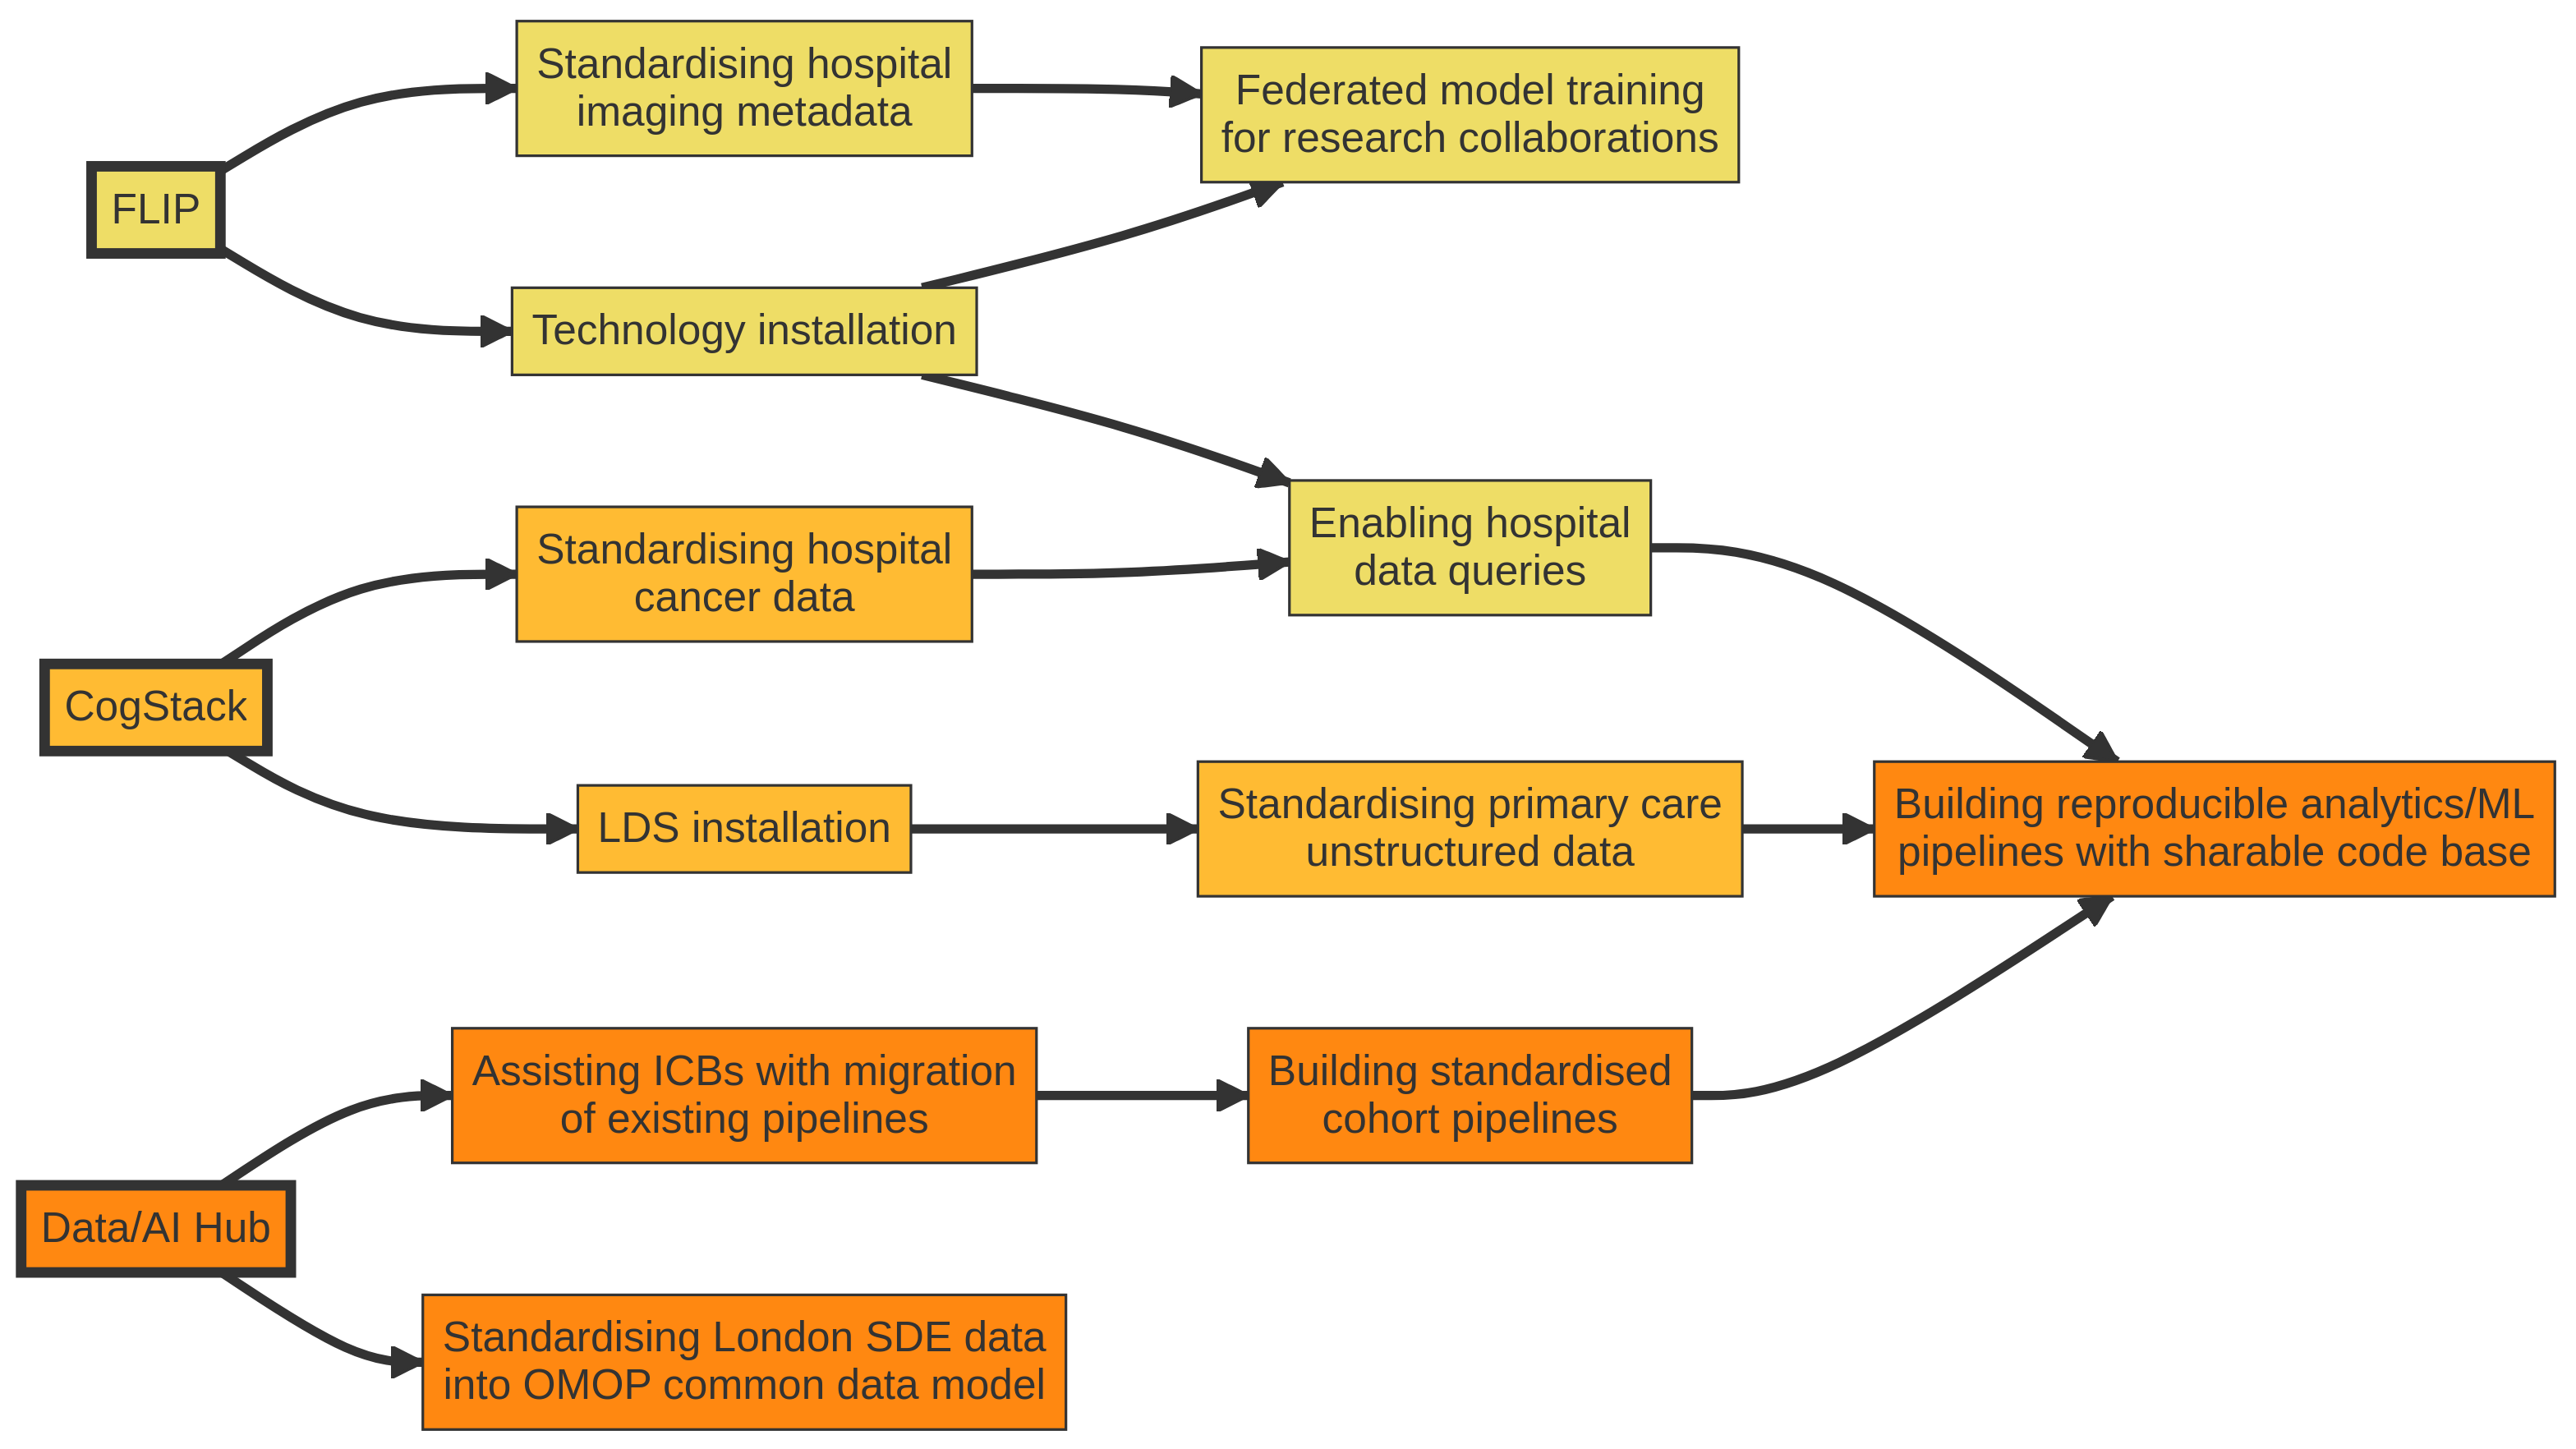
\includegraphics[width=6in,height=3.38in]{index_files/figure-latex/mermaid-figure-8.png}

}

\caption{\label{fig-aic-objectives}Summary of AIC work components and
objectives. FLIP = Federated Learning and Interoperability Platform; ML
= Machine Learning.}

\end{figure}%

\textsubscript{Source:
\href{https://d3london.github.io/sde_aic_docs/index.qmd.html}{Article
Notebook}}

As the LDS ICB environments share a common data model, any pipelines
created in collaboration with an ICB can be adapted and used for any
other ICB (or deployed across multiple environments to create pan-London
insights). This will also facilitate the use of shared terminologies,
and validating / versioning / serving NHS-owned machine learning models
across regions.

\subsection{Proposed use-cases}\label{proposed-use-cases}

The following three use-cases are \emph{examples} of analytics projects
that can be supported within the SDE ecosystem, in collaboration between
ICB/NHS analytics teams and the AIC/SDE team. Use-cases align to the
London Health Data Strategy and long term condition priorities, as well
as national programmes such as CORE20PLUS5, and are proposed here
following early discussions with London ICBs. An objective for any work
is to build upwards from a foundation of reproducible pipelines, towards
data science and predictive analytics
(Figure~\ref{fig-general-framework}).

\begin{figure}

\centering{

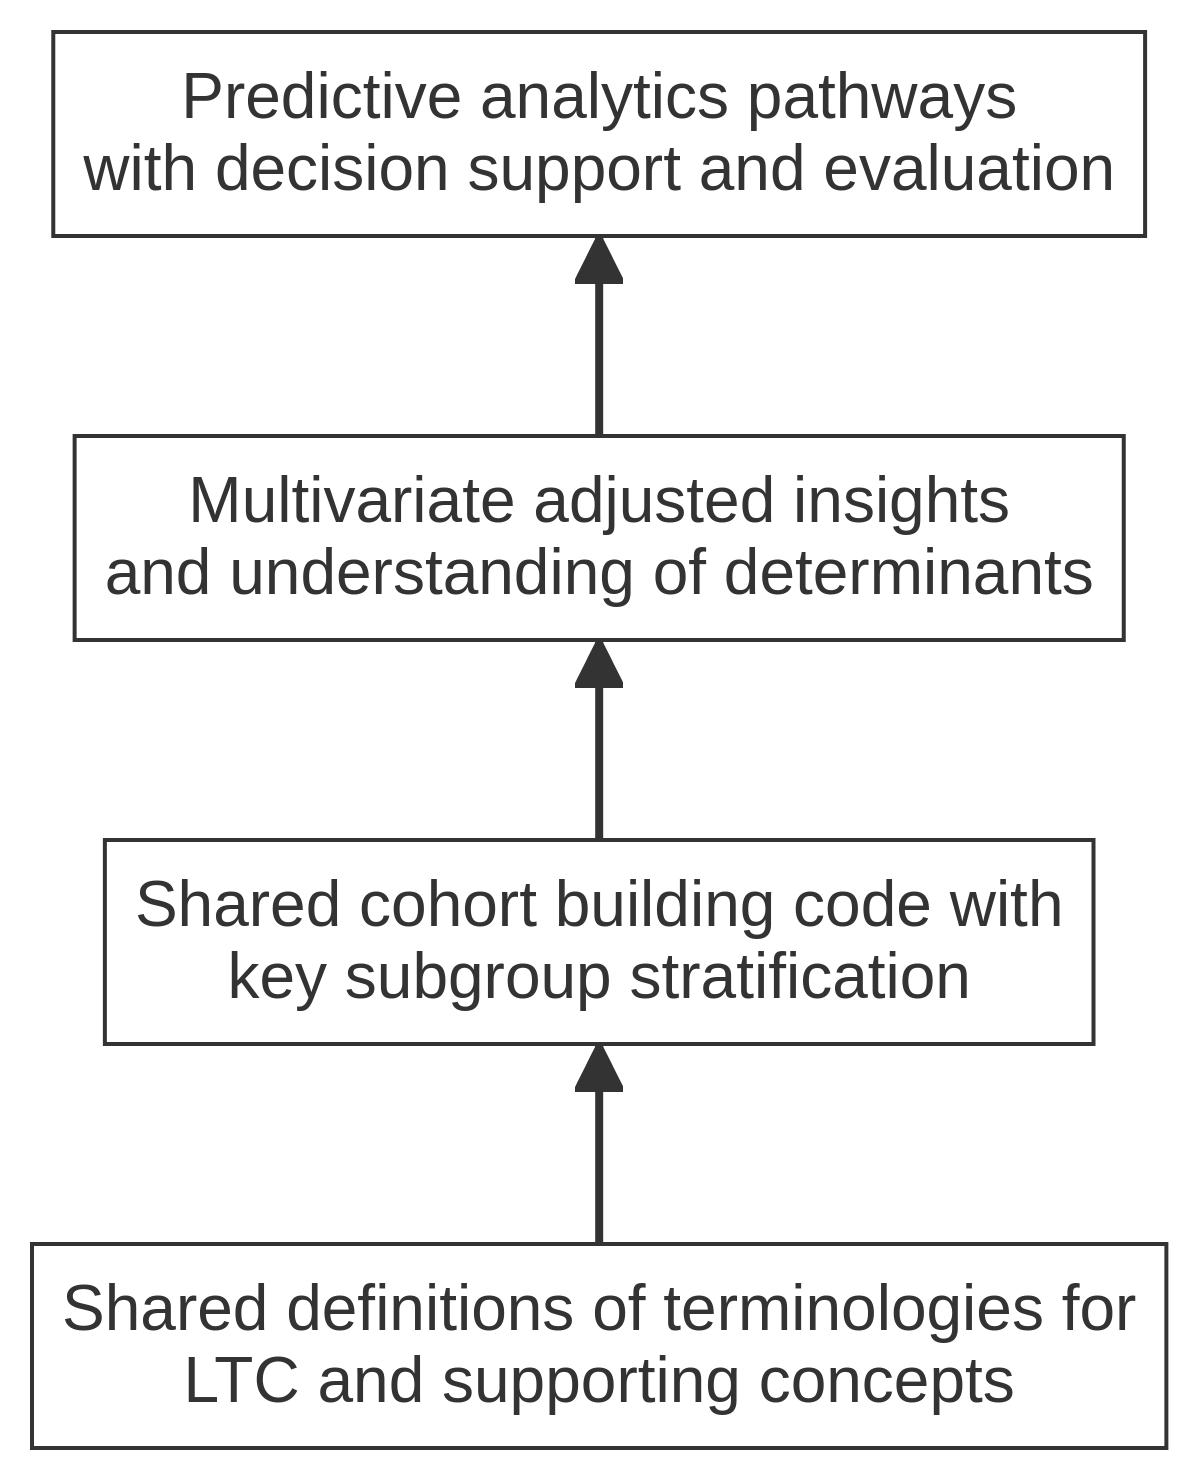
\includegraphics[width=6in,height=7.41in]{index_files/figure-latex/mermaid-figure-7.png}

}

\caption{\label{fig-general-framework}General framework for use-cases:
moving towards advanced analytics}

\end{figure}%

\textsubscript{Source:
\href{https://d3london.github.io/sde_aic_docs/index.qmd.html}{Article
Notebook}}

\subsubsection{Systematic measurement of group and individual health
inequality}\label{systematic-measurement-of-group-and-individual-health-inequality}

\textbf{AIM:} To systematically surface multiple dimensions of health
inequality across sociodemographic / geospatial groups, and across
individual patients, and to monitor this data continuously across key
long-term conditions.

\textbf{SUMMARY:} Health inequality refers to measurable differences in
health outcomes and determinants between individuals or groups
(e.g.~morbidity, co-morbidity, disease complications/death, healthcare
access, disease screening, treatment delivery). Where there is health
inequality, the principle of health \emph{equity} emphasises the
recognition and reduction of disparities in determinants.

Health inequality is traditionally measured and visualised as a
comparison of prevalence/incidence across different population groups.
While helpful for broad insights, this offers limited understanding of
complex individual circumstances. Instead, measurement of inequalities
can be extended to individual patients, by using clinical domain
knowledge to define `indicators' of unequal disease, diagnosis, and
treatment pathways. For example, in an individual with a long-term
condition (LTC), indicators of inequality can include:

\begin{longtable}[]{@{}
  >{\raggedright\arraybackslash}p{(\columnwidth - 0\tabcolsep) * \real{1.0000}}@{}}
\toprule\noalign{}
\endhead
\bottomrule\noalign{}
\endlastfoot
1. LTC surfacing at an early age (Figure~\ref{fig-onset-time}) \\
2. LTC in proximity to relevant co-morbidities (e.g.~cardiovascular risk
factors) \\
3. Diagnosis at a \emph{late} age but with more severe disease (e.g.~in
Diabetes, measured by HbA1c or presence of end-organ complications) \\
4. Reduced health engagement/encounters/treatment compared to what is
expected based on disease severity \\
5. Shorter time to complications and mortality following diagnosis \\
\end{longtable}

The contribution of individual indicators to later outcomes can be
measured in multivariate statistical models, and used to understand
inequality determinants for any given individual. Determinants can be
visualised for small specific groups, or individuals, with comparison to
`what is expected' in a background population. The result is an increase
in actionability.

\begin{figure}

\centering{

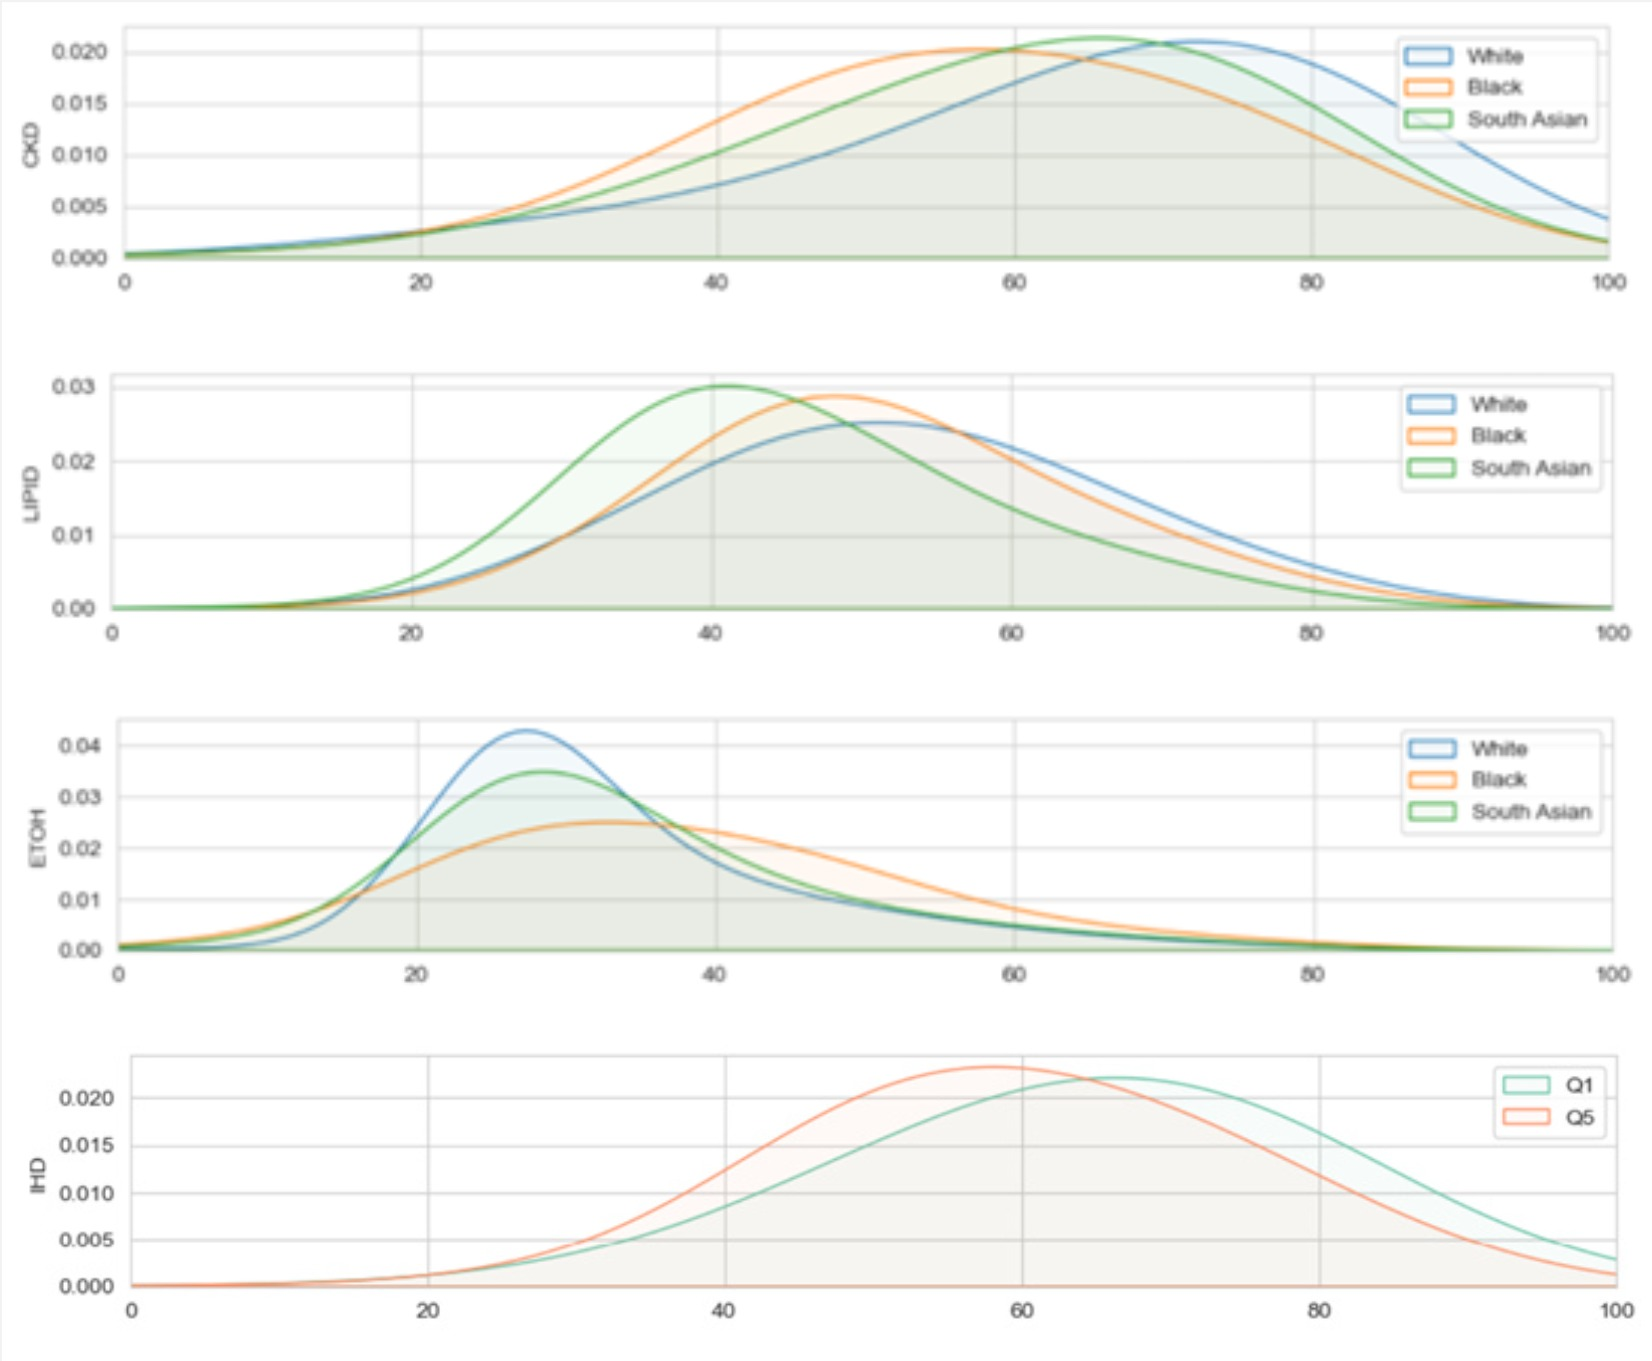
\includegraphics{media/onset_over_time.jpg}

}

\caption{\label{fig-onset-time}Inequality in age of onset across
demographic groups and deprivation, generated automatically through
input of condition and group for stratification}

\end{figure}%

As per the framework described in (Figure~\ref{fig-general-framework}),
the initial stage of work will include defining shared terminologies,
concepts, and indicators that cover long-term conditions of interest.
Secondly, existing descriptions of health inequality can be migrated
onto the LDS environment using shared terminologies and concepts, such
that any condition can be repreducibly visualised across multiple
dimensions and `cuts'. This foundation can be extended to encompass
specific inequality indicators and statistical insights, at a small
group and individual level, and the use of these insights to identify
patients at greatest risk of health inequality, or those with
addressable inequities.

\subsubsection{Cardiovascular disease prevention through decision
intelligence}\label{cardiovascular-disease-prevention-through-decision-intelligence}

\textbf{AIM:} To enhance descriptive population health management with
explainable predictive analytics and clinical guideline-based ``decision
intelligence'' systems, across cardiovascular related co-morbidities
(including hypertension, diabetes, chronic kidney disease).

\textbf{SUMMARY:} The spectrum of cardiovascular long-term conditions
(LTC) and associated risk factors is wide, and includes hypertension,
diabetes, obesity, high cholesterol, ischaemic heart disease, stroke,
and chronic kidney disease, as well as dementia, atrial fibrillation,
and heart failure. The burden of such diseases is high.
\href{https://cks.nice.org.uk/topics/cvd-risk-assessment-management/background-information/burden-of-cvd/}{Heart
disease} alone causes a quarter of deaths in the UK, with direct costs
to the healthcare system estimated at £9 billion by the British Heart
Foundation. Cardiovascular disease is seen as a
\href{https://imperialcollegehealthpartners.com/portfolio/onelondon/}{priority
area for use of data} across OneLondon patient and public engagement.

\begin{figure}

\centering{

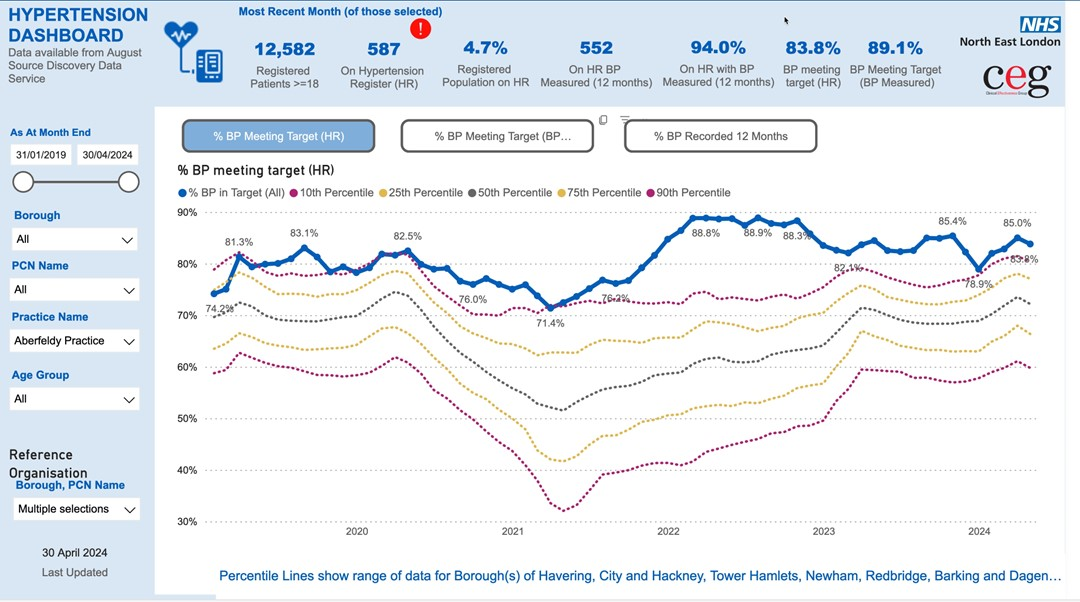
\includegraphics{media/example_dashboard.jpg}

}

\caption{\label{fig-icb-hypertension}Existing ICB dashboard for
Hypertension}

\end{figure}%

In London ICBs, there is robust aggregate understanding of LTC, through
prevalence reporting and Quality Outcome Framework (QOF) indicators.
Existing ICB dashboards (Figure~\ref{fig-icb-hypertension}) show how a
practice or a system are performing relative to their peers. However,
such reporting has limitations, including: (1) lack of adjustment for
demographics and other confounding variables; (2) difficulty in
surfacing individual patients with direct actions; and (3) lack of
consideration of co-morbidities - as multi-morbidity tends to change the
risk profile and urgency of response for individuals. Some of these
limitations are being addressed by existing work in London pathfinder
programmes, and in other regions such as Greater Manchester, which are
moving towards electronic identification of patients who may be actioned
via pre-agreed clinical pathways
(Figure~\ref{fig-simple-pathway-action}).

\begin{figure}

\centering{

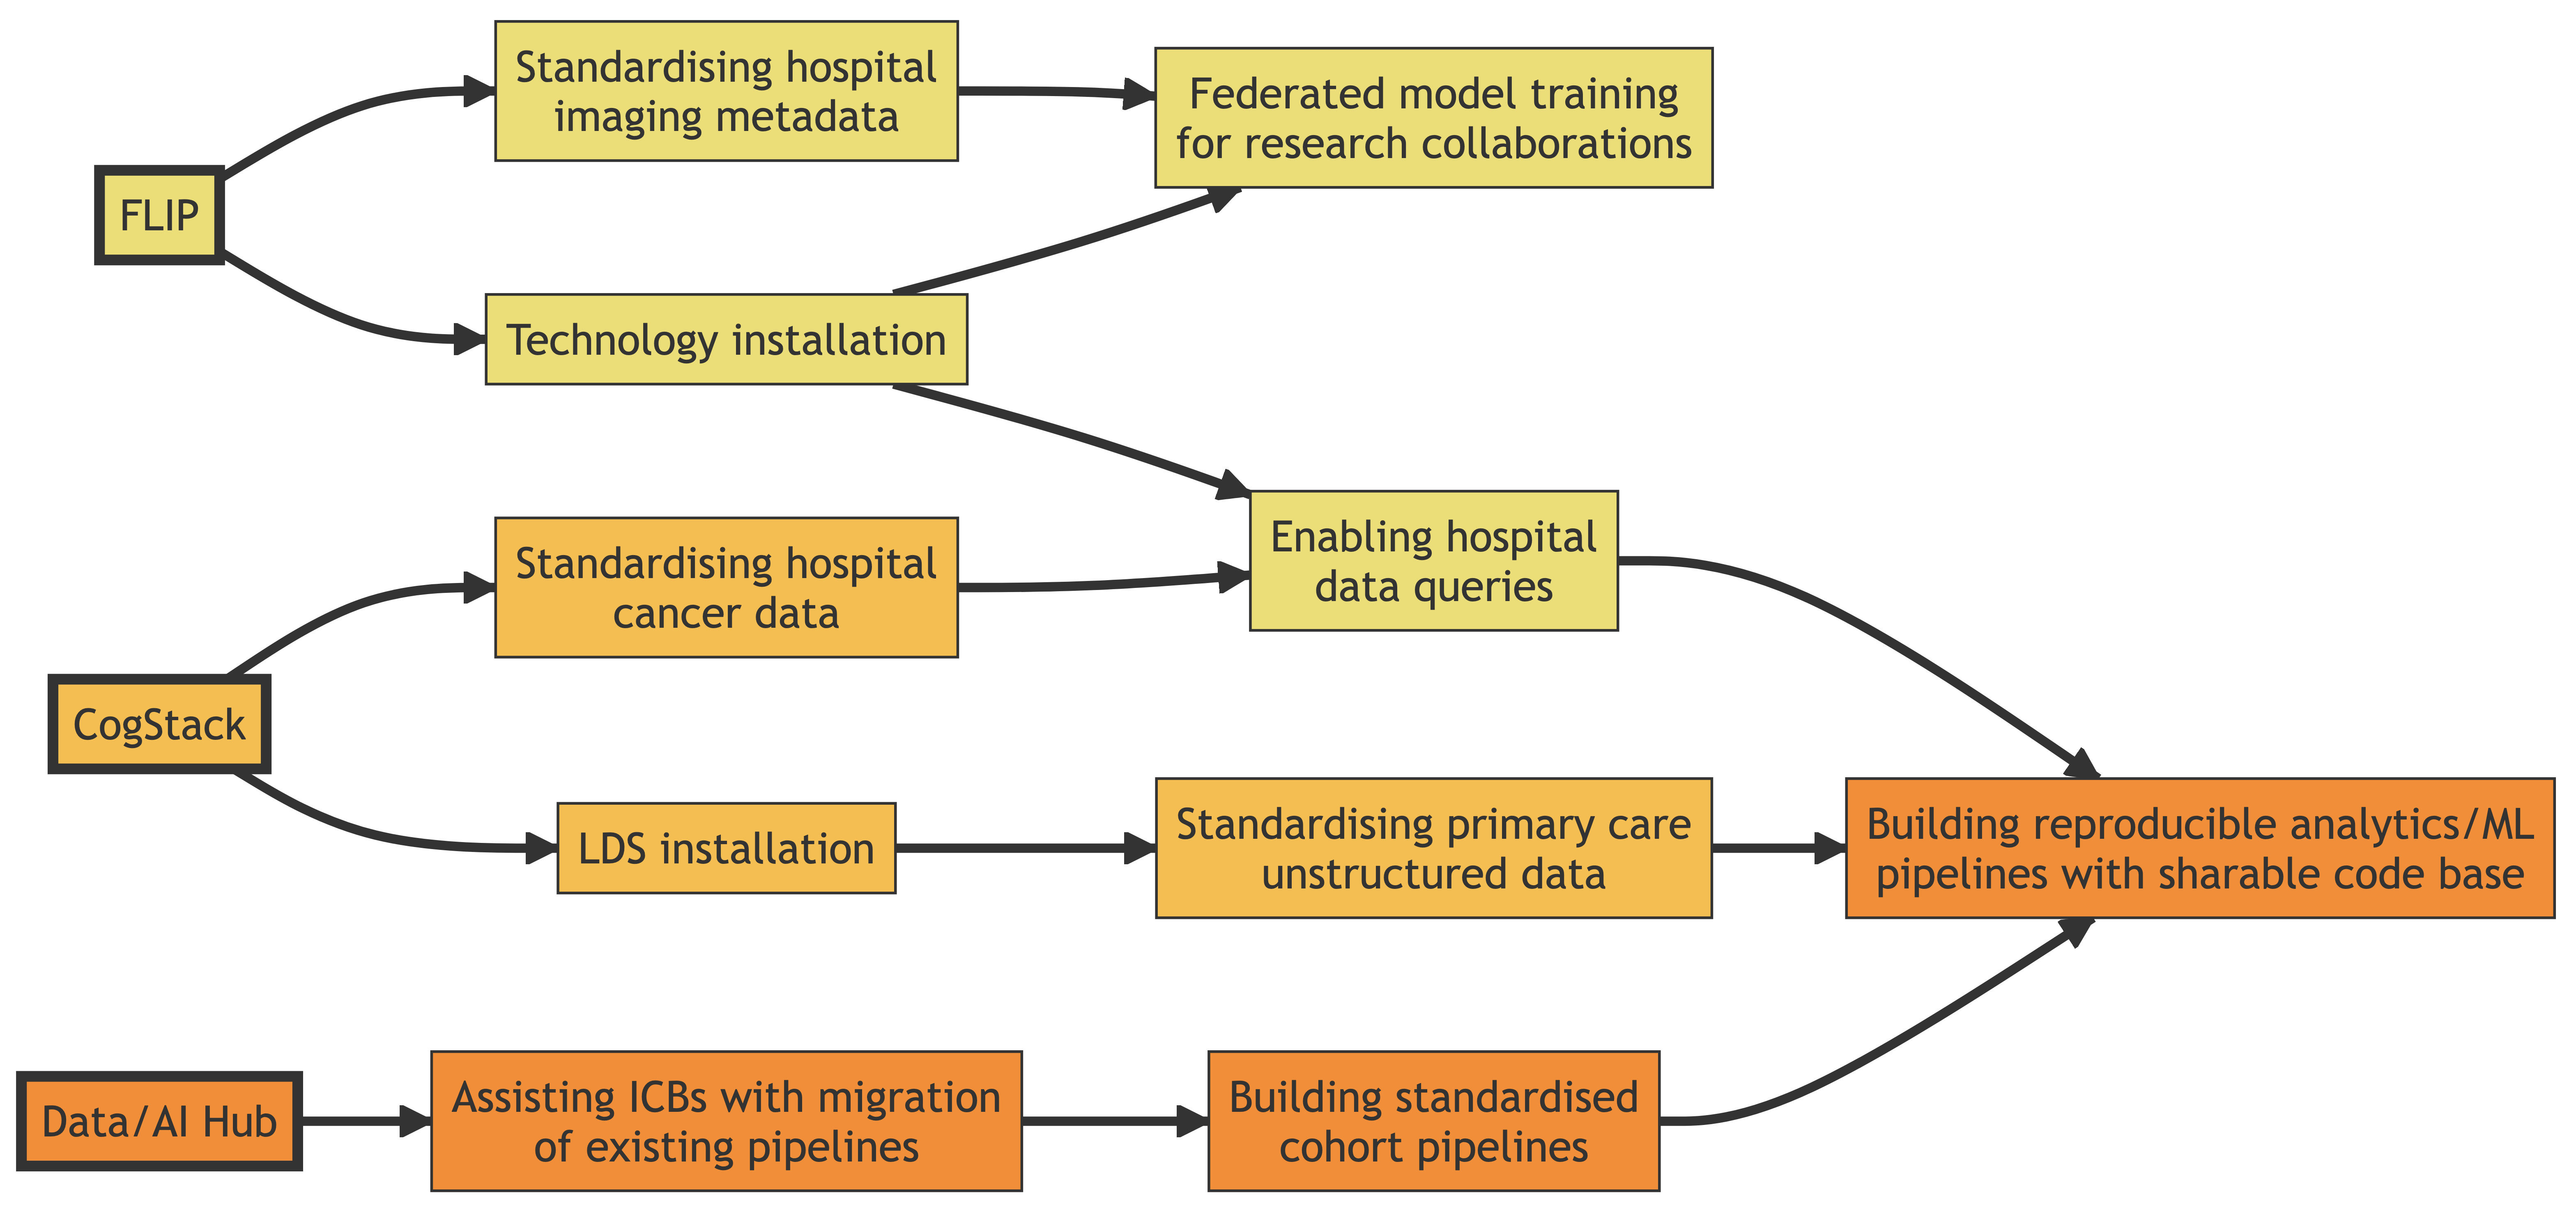
\includegraphics[width=6in,height=2.51in]{index_files/figure-latex/mermaid-figure-6.png}

}

\caption{\label{fig-simple-pathway-action}Examples of simple logical
triggers leading to clinical actions. CKD = Chronic Kidney Disease; BB =
Beta-blocker; ACEi = ACE inhibitor.}

\end{figure}%

\textsubscript{Source:
\href{https://d3london.github.io/sde_aic_docs/index.qmd.html}{Article
Notebook}}

These limitations can be surmounted through using richer data to
generate personalised risk profiles for individual patients (rather than
aggregate group summaries). A previous collaboration between the AIC and
North-East London ICB was able to develop precise cardiovascular risk
prediction models for individuals, using explainable machine-learning
algorithms and the linked patient health record. Actionable factors
could also be highlighted in patients with high risk, with their
relative importance explained through statistical modelling to enhance
explainability (Figure~\ref{fig-htn-actionable}).

\begin{figure}

\centering{

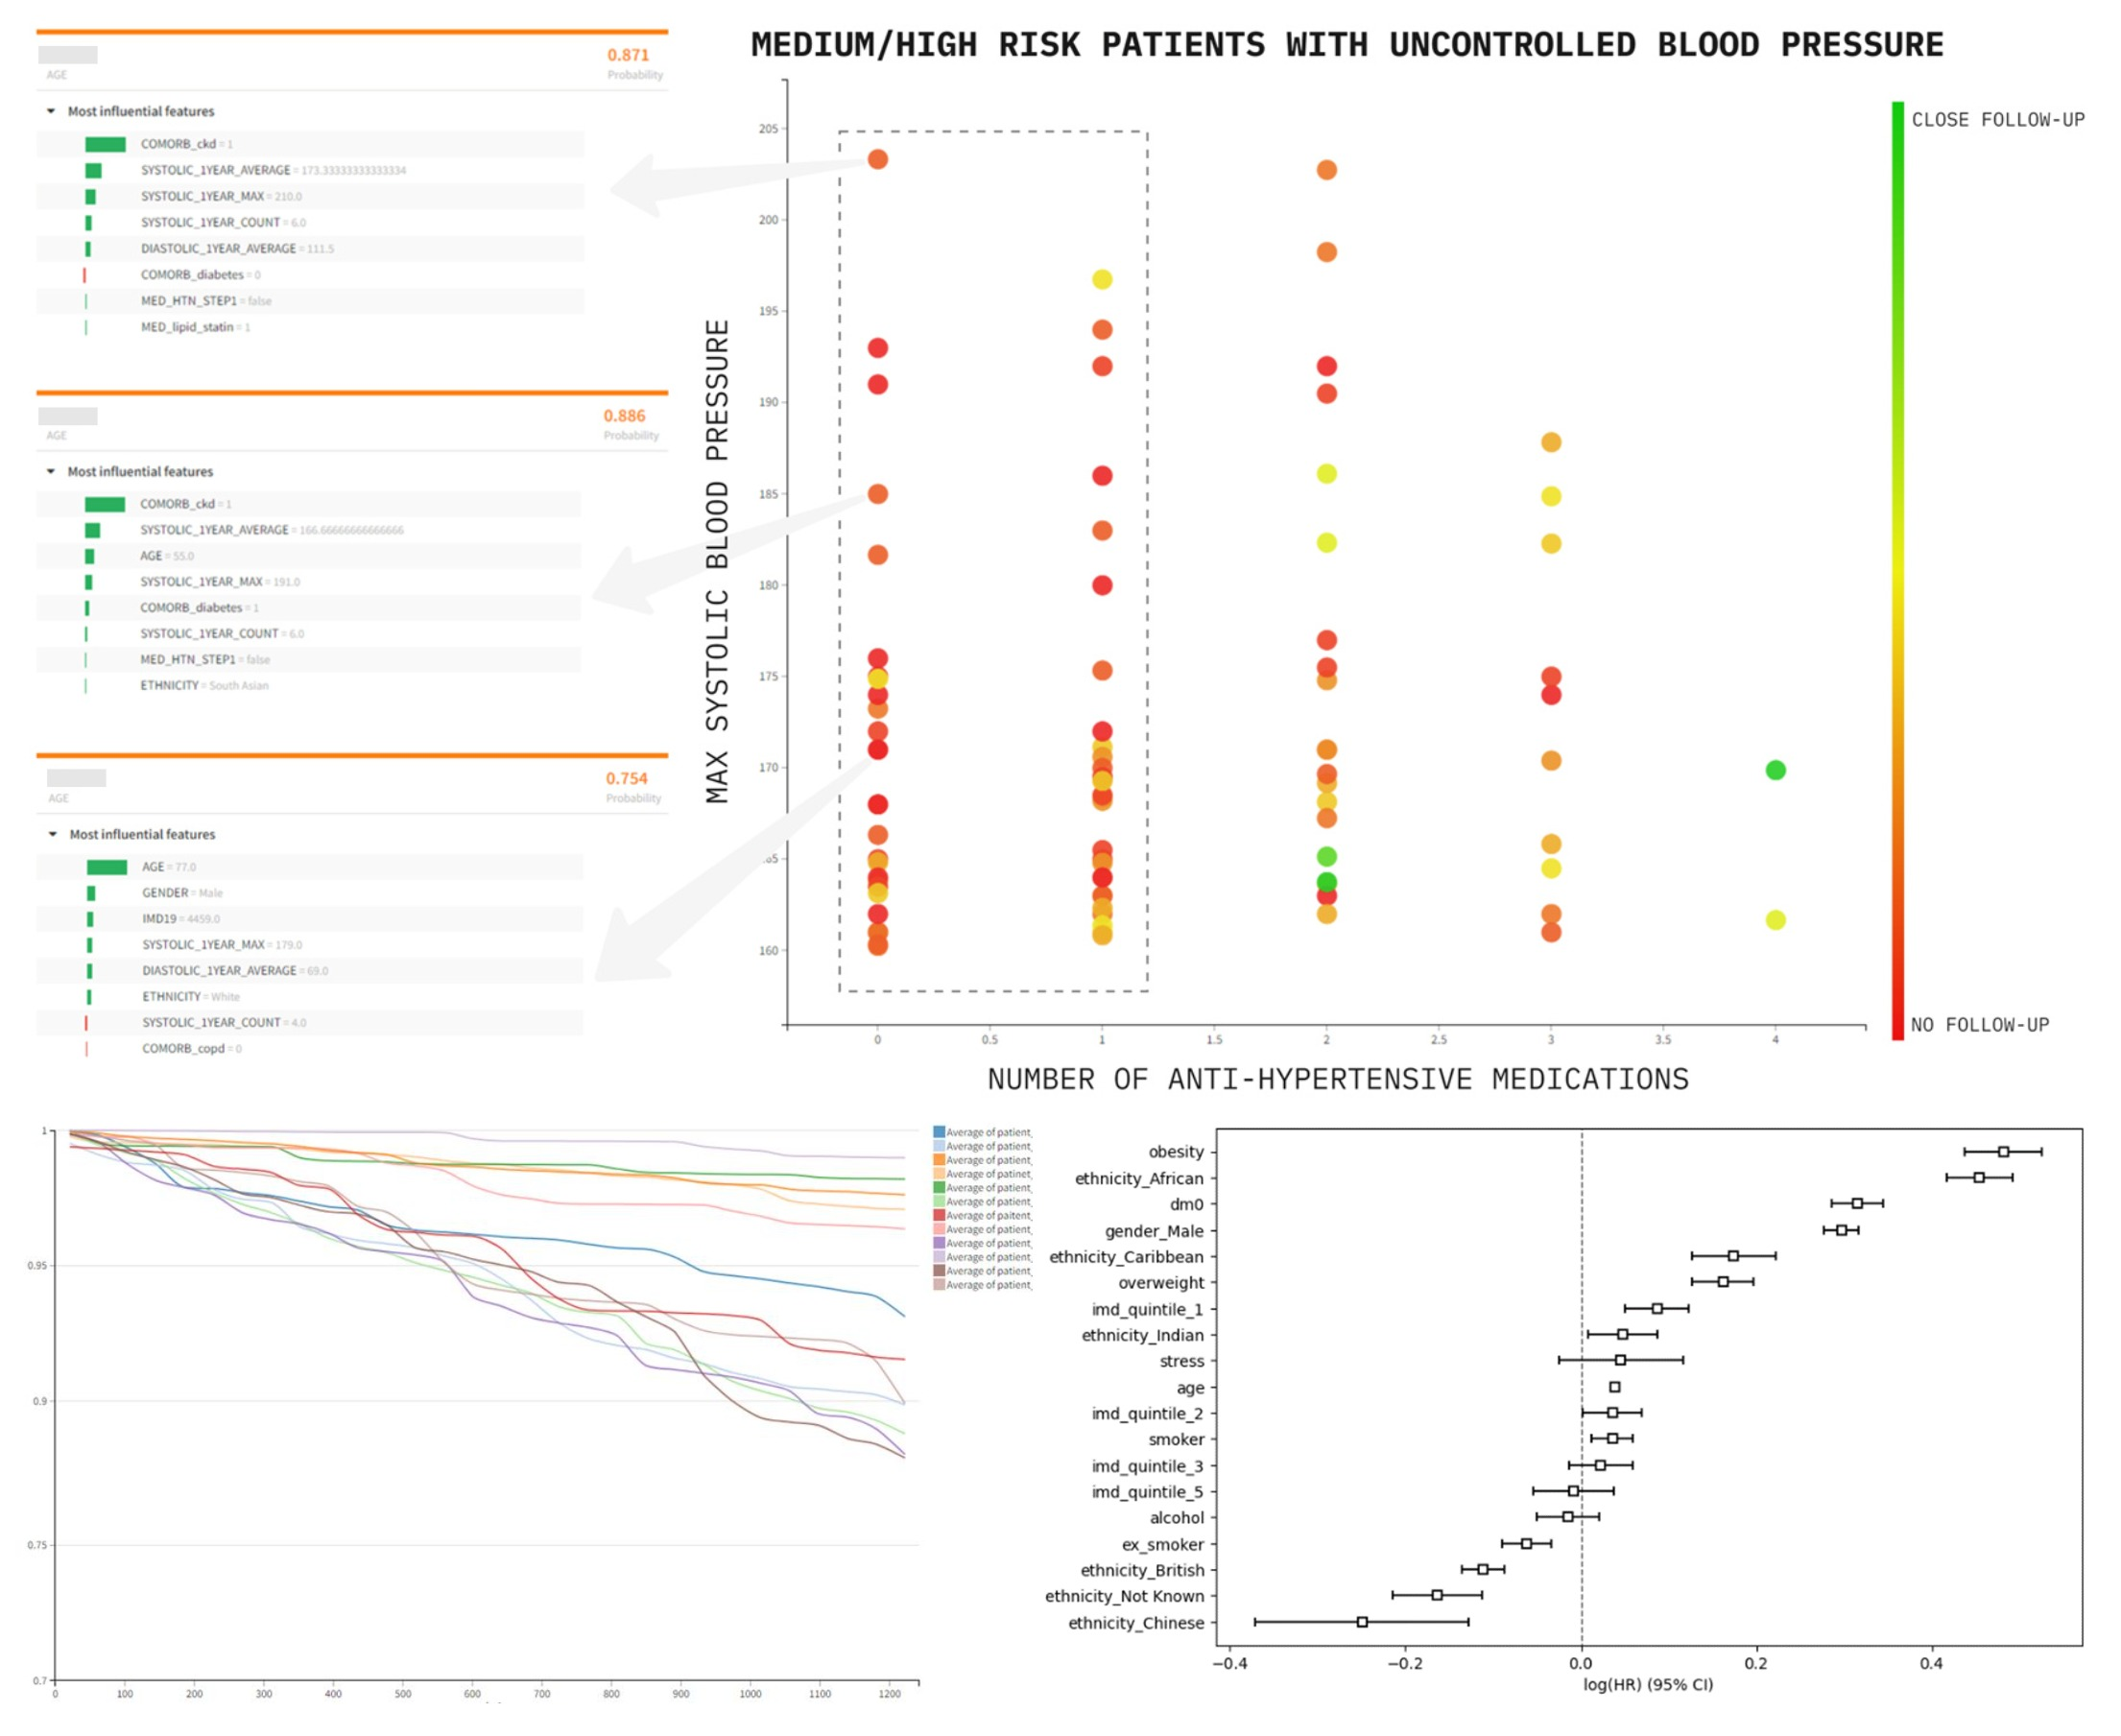
\includegraphics{media/htn_actionable.jpg}

}

\caption{\label{fig-htn-actionable}Actionable factors (including
follow-up, treatment, blood pressure control) and association of
features with adverse outcome in high risk hypertensive patients}

\end{figure}%

Predictive analytics alone is not a solution. Being ``high risk'' alone
may be difficult to action clinically, and may not lead to improved care
or prevention. Instead, it is possible to use clinical guidelines and
domain knowledge to identify specific optimisation or preventative
actions (much like Figure~\ref{fig-simple-pathway-action}) but
systematically, and on a larger scale. The combination of personalised
risk profiles and personalised actionability for supporting decisions,
is referred to as ``decision intelligence''.

This use-case will again aim to develop shared terminologies, features,
and code to enhance current pipelines and dashboards. In addition,
collaboration extend these through:

\begin{enumerate}
\def\labelenumi{(\arabic{enumi})}
\item
  Computerisation of Quality Outcomes Framework targets and clinical
  guidelines, in conjunction with local clinical teams, to develop safe
  decision logic for use in the ``effector'' arm.
\item
  Use of CogStack to extract additional valuable context and missing
  codes from unstructured text.
\item
  Use rich features in the EHR to develop statistical and machine
  learning models for predicting and understanding risk of progression
  across range of cardiovascular morbidity and co-morbidity.
\item
  For given patient's health record, understand actions (i.e.~are there
  actions available, and what are they) combined with explainable risks
  across multiple conditions (i.e.~what are the highest risks for this
  patient and why).
\item
  Return individual patient insights and suggested actions to clinical
  systems
\end{enumerate}

Highly individualised patient profiles is the objective of
``personalised care'', and is required to move towards preventative
healthcare. Additional work is being conducted to explore pushing
insights directly to Electronic Health Records. Any deployed systems
will need to be evaluated and monitored for safety and fairness, with a
process of training and handover to continuity teams following the end
of this SDE programme phase.

\subsubsection{Joining up cancer
pathways}\label{joining-up-cancer-pathways}

\textbf{AIM:} To link cancer pathways (including screening, diagnosis,
staging, and outcomes) across primary care and secondary care. To
identify areas of inequality and late diagnosis, and to generate
predictive insights for risk and screening recall.

\textbf{BACKGROUND:}

\textbf{APPROACH:}

\subsection{Next steps}\label{next-steps}

\ldots{}



\end{document}
